\section{Análisis}
\section{Reglas de negocio}

% ===============================
% 1. Reglas de inicialización y coherencia
% ===============================

\begin{frame}{Reglas de negocio}
	\begin{enumerate}[label=RN\arabic*.]
		\item Para iniciar la simulación es necesario que el conjunto de estados, la topología de la vecindad, la condición de frontera y la función de transición hayan sido definidos.
		
		\item Una vez iniciada la simulación, no se puede cambiar el conjunto de estados, la topología de la vecindad ni la función de transición.
		
		\item El estado de una celda en el tiempo $t+1$ depende únicamente de su estado actual y de los estados de sus vecinos.
	\end{enumerate}
\end{frame}

% ===============================
% 2. Reglas sobre interacción con la simulación
% ===============================

\begin{frame}{Reglas de negocio}
	\begin{enumerate}[label=RN\arabic*.]
		\setcounter{enumi}{3}
		
		\item El usuario puede manipular el estado de una celda y las condiciones de frontera en tiempo de ejecución.
		
		\item El usuario puede pausar, detener, reanudar o retroceder la simulación sin pérdida de información.
		
		\item Solo se permite una simulación activa por sesión.
	\end{enumerate}
\end{frame}

% ===============================
% 3. Reglas sobre importación/exportación
% ===============================

\begin{frame}{Reglas de negocio}
	\begin{enumerate}[label=RN\arabic*.]
		\setcounter{enumi}{6}
		
		\item Los datos importados deben cumplir con el formato definido por el sistema para garantizar su correcta interpretación.
		
		\item Los datos exportados deben conservar el mismo formato que los datos importados.
	\end{enumerate}
\end{frame}


% ======================================================
% REQUISITOS FUNCIONALES
% ======================================================

\section{Requisitos funcionales}

% ===============================
% 1. Interacción con el espacio celular
% ===============================

\begin{frame}{Requisitos funcionales}
	\begin{enumerate}[label=RF\arabic*.]
		\item El sistema debe mostrar una cuadrícula regular y finita que represente el espacio celular.
		
		\item El sistema debe permitir al usuario interactuar con el espacio celular, asignando o modificando los estados de las celdas.
		
		\item El sistema debe permitir al usuario definir el conjunto de estados, la topología de la vecindad y las condiciones de frontera.
		
		\item El sistema debe permitir la evolución del espacio celular mediante un único paso o de forma continua, ajustando la velocidad de actualización.
	\end{enumerate}
\end{frame}

% ===============================
% 2. Importación/exportación y módulo neuronal
% ===============================

\begin{frame}{Requisitos funcionales}
	\begin{enumerate}[label=RF\arabic*.]
		\setcounter{enumi}{4}
		
		\item El sistema debe permitir la importación y exportación de configuraciones y evoluciones del espacio celular.
		
		\item El sistema debe permitir al usuario establecer la función de transición manualmente.
		
		\item El sistema debe permitir configurar una red neuronal para imitar la evolución de un autómata celular dada una trayectoria objetivo.
		
		\item El sistema debe entrenar una red neuronal con los parámetros proporcionados por el usuario para replicar dicha evolución.
	\end{enumerate}
\end{frame}

\begin{frame}{Diagrama de casos de uso}
	\begin{figure}[H]
		\centering
		\begin{tikzpicture}
			\node[fill=white, inner sep=0pt] {
				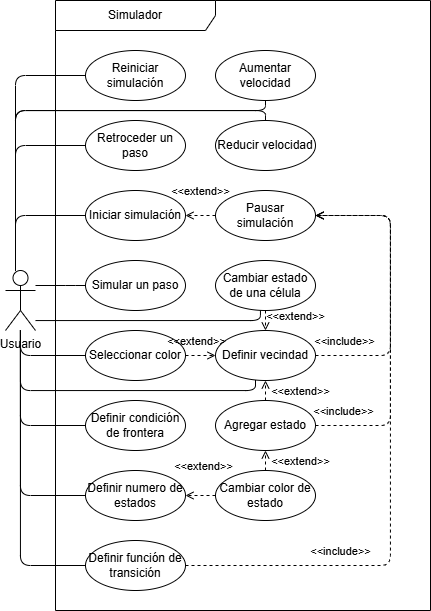
\includegraphics[width=0.3\linewidth]{images/uml_ucd.png}
			};
		\end{tikzpicture}
		\caption{Diagrama de casos de uso.}
	\end{figure}
\end{frame}


